\documentclass[tikz,border=2pt]{standalone}
% Preámbulo común de los diagramas TikZ (misma paleta y letra que las notas)
\usepackage[T1]{fontenc}\usepackage[utf8]{inputenc}
\usepackage{libertinus}\usepackage{libertinust1math}
\usepackage[defaultsans,scale=0.92]{lato}
\usepackage{amsmath,amssymb,bm}
\usepackage{tikz}\usetikzlibrary{calc,positioning,arrows.meta,shapes.geometric,decorations.pathreplacing,decorations.pathmorphing,fit,backgrounds}
\definecolor{snlazul}{HTML}{1E5AA8}\definecolor{snlnoche}{HTML}{14213D}\definecolor{snlvioleta}{HTML}{6C4AB6}
\definecolor{snlcoral}{HTML}{D1495B}\definecolor{snlambar}{HTML}{E09F3E}\definecolor{snlverde}{HTML}{2A9D8F}
\definecolor{snlteal}{HTML}{0F7173}\definecolor{snlgris}{HTML}{5C677D}\definecolor{snlfondo}{HTML}{F4F6FA}
\tikzset{>={Stealth[length=2.2mm]},
  bloque/.style={draw=#1,fill=#1!8,thick,rounded corners=2pt,minimum height=11mm,minimum width=20mm,align=center,font=\small},
  bloque/.default=snlazul,
  suma/.style={draw=snlnoche,thick,circle,inner sep=0pt,minimum size=5mm},
  flecha/.style={->,thick,draw=snlnoche},
  etq/.style={font=\small,text=snlnoche},
  nota/.style={font=\footnotesize\sffamily,text=snlgris,align=center}}

\begin{document}
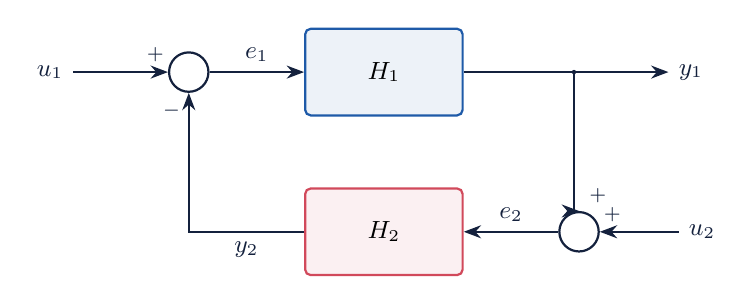
\begin{tikzpicture}[node distance=12mm]
 \node[suma] (s1) {};
 \node[bloque=snlazul,right=12mm of s1] (H1) {$H_1$};
 \node[bloque=snlcoral,below=9mm of H1] (H2) {$H_2$};
 \node[suma,right=12mm of H2] (s2) {};
 \draw[flecha] ($(s1.west)+(-12mm,0)$) node[left,etq]{$u_1$} -- (s1);
 \draw[flecha] (s1) -- node[above,etq]{$e_1$} (H1);
 \draw[flecha] (H1.east) -- ++(26mm,0) node[right,etq]{$y_1$};
 \draw[flecha] ($(H1.east)+(14mm,0)$) |- (s2.north) ;
 \draw[flecha] ($(s2.east)+(10mm,0)$) node[right,etq]{$u_2$} -- (s2);
 \draw[flecha] (s2) -- node[above,etq]{$e_2$} (H2);
 \draw[flecha] (H2.west) -| node[pos=0.25,below,etq]{$y_2$} (s1.south);
 \node[font=\scriptsize,text=snlnoche] at ($(s1.south)+(-2.2mm,-2.2mm)$) {$-$};
 \node[font=\scriptsize,text=snlnoche] at ($(s1.west)+(-1.6mm,2.2mm)$) {$+$};
 \node[font=\scriptsize,text=snlnoche] at ($(s2.north)+(2.4mm,2.0mm)$) {$+$};
 \node[font=\scriptsize,text=snlnoche] at ($(s2.east)+(1.6mm,2.2mm)$) {$+$};
 \fill[snlnoche] ($(H1.east)+(14mm,0)$) circle (0.8pt);
\end{tikzpicture}
\end{document}
